%! Author = mariuszindel
%! Date = 02.11.20

\section{Reflection}

\subsection{Überblick}
\subsubsection{Anwendung}
\begin{itemize}
    \item Type Discovery
    \begin{itemize}
        \item Suchen und Instanzieren von Typen
        \item Zugriff auf dynamische Datenstrukturen (z.B. auf JavaScript-Objekte)
    \end{itemize}
    \item Late Binding (Methods / Properties)
    \begin{itemize}
        \item Aufruf von Methoden / Properties nach Type Discovery
    \end{itemize}
    \item Reflection Emit / Code-Emittierung
    \begin{itemize}
        \item Erstellen von Typen inkl. Members zur Laufzeit
    \end{itemize}
\end{itemize}

\subsubsection{Klasse «System.Type»}
\begin{itemize}
    \item Alle Typen in der Common Language Runtime CLR sind selbst-definierend
    \item Klasse «System.Type»
    \begin{itemize}
        \item Einstiegspunkt aller Reflection-Operationen
        \item Representiert einen Typen mit all seinen Eigenschaften
        \item Abstrakte Basisklasse
        \item «System.RuntimeType» wird jeweils verwendet
        \item Alle Objekte sind Instanzen von Typen
        \item Vererbungs-Hierarchien sind auch abgebildet
    \end{itemize}
\end{itemize}
\vspace{-8pt}
\begin{center}
    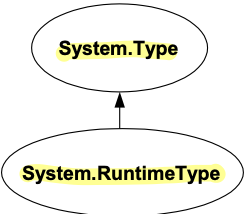
\includegraphics[scale=.38]{graphic/ref attr/System.Type.png}
\end{center}
\vspace{-8pt}

\subsubsection{typeof / GetType()}
Ermitteln von «System.Type» via
\begin{itemize}
    \item «obj».GetType()
    \item typeof(«classname»)
\end{itemize}
\vspace{-8pt}
\begin{center}
    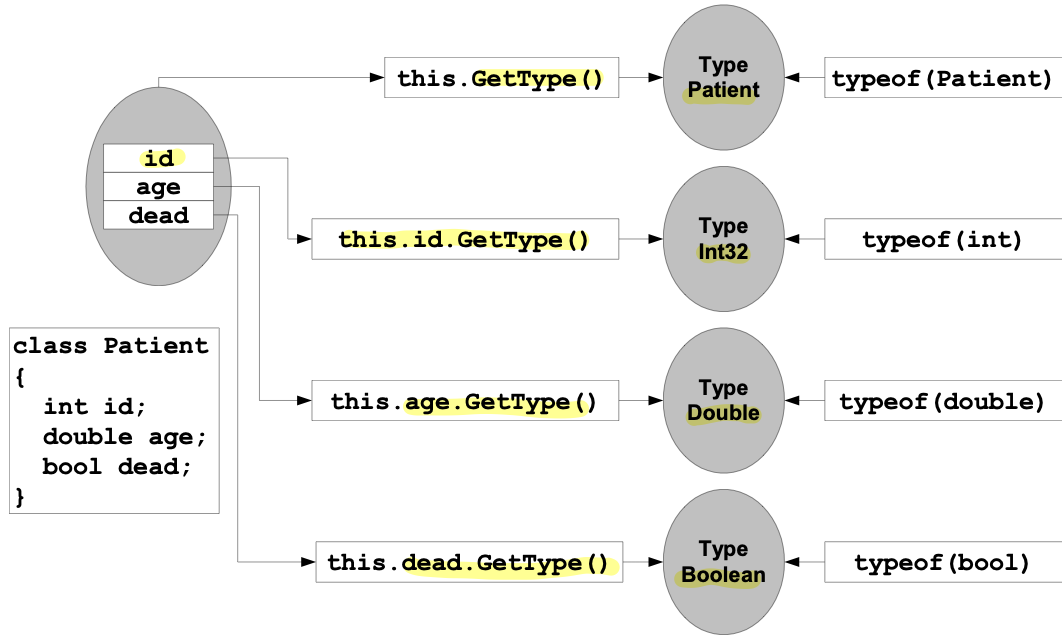
\includegraphics[scale=.35]{graphic/ref attr/typeof.png}
\end{center}
\vspace{-8pt}
«System.Type» beschreibt sich selbst als «System.Type» Objekt

\begin{center}
    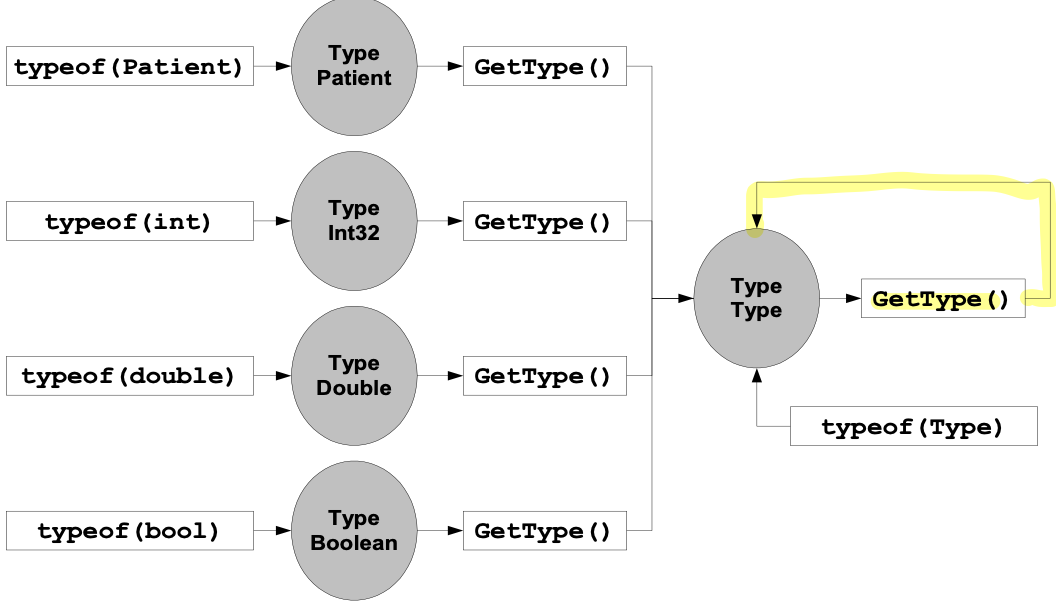
\includegraphics[scale=.35]{graphic/ref attr/typeof2.png}
\end{center}
\vspace{-8pt}

\subsubsection{Member-Informationen / Typ-Hierarchie}
\begin{itemize}
    \item Jeder Klassen-Member hat einen eigenen Reflection-Typen
    \item «System.Runtime.MemberInfo» ist abstrakte Basisklasse für Members
    \item Suche von Members
    \begin{itemize}
        \item Allgemein z.B. nach Sichtbarkeit «public»
        \item Nach bestimmter Member-Art z.B. alle Properties
    \end{itemize}
    \item Nicht-zugreifbare Members auch einsehbar (z.B. private Felder)
    \item Klassen befinden sich in
    \begin{itemize}
        \item Assembly
        \item Namespace
    \end{itemize}
\end{itemize}
\vspace{-8pt}
\begin{center}
    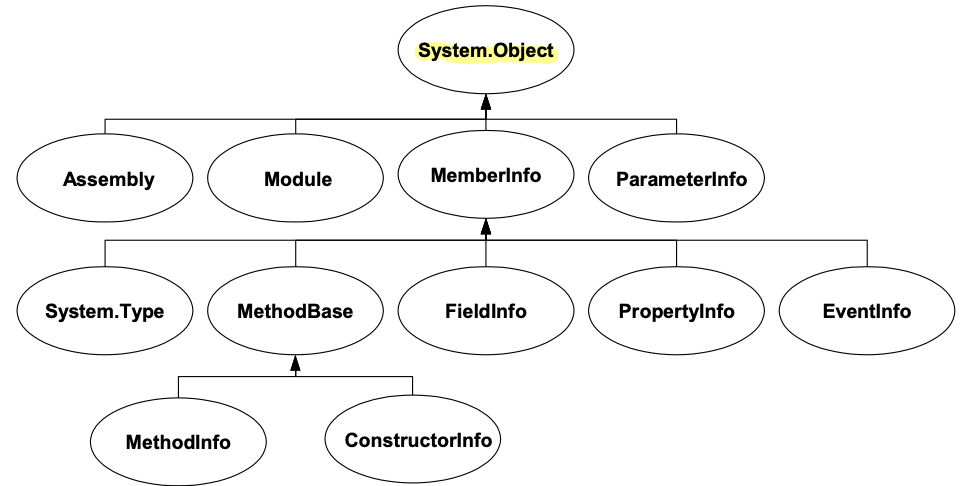
\includegraphics[scale=.35]{graphic/ref attr/Member-Informationen Typ-Hierarchie.png}
\end{center}
\vspace{-8pt}


\subsection{Metadaten}

\subsubsection{Type-Discovery}
Suche aller Typen in einem Assembly
\begin{lstlisting}
Assembly a01 = Assembly.Load("mscorlib");

Type[] t01 = a01.GetTypes();
foreach (Type type in t01) {
    Console.WriteLine(type);
    MemberInfo[] mInfos = type.GetMembers();
    foreach (var mi in mInfos) {
        Console.WriteLine(
        "\t{0}\t{1}",
        mi.MemberType,
        mi);}}

//Ausgabe:
System.Int32
    Method Int32 CompareTo(System.Object)
    Method Int32 CompareTo(Int32)
    ...
\end{lstlisting}

\subsubsection{Members auslesen / Alle}
Suche aller Members eines Typen
\begin{lstlisting}
Type type = typeof(Counter);

MemberInfo[] miAll = type.GetMembers();
foreach (MemberInfo mi in miAll) {
    Console.WriteLine("{0} is a {1}",
        mi, mi.MemberType);}

Console.WriteLine("----------");

PropertyInfo[] piAll = type.GetProperties();
foreach (PropertyInfo pi in piAll) {
    Console.WriteLine("{0} is a {1}",
        pi, pi.PropertyType);}

//Ausgabe:
Int32 get_CountValue() is a Method
Void set_CountValue(Int32) is a Method
Void Increment() is a Method
Int32 GetHashCode() is a Method Type
Void .ctor(Int32) is a Constructor
Int32 CountValue is a Property
PropertyChangedEventHandler PropertyChanged is a Event
----------
Int32 CountValue is a Property
\end{lstlisting}

\subsubsection{Members auslesen / Dynamisch}
Suche spezieller Members eines Typen
\begin{lstlisting}
Type type = typeof(Assembly);


BindingFlags bf =
    BindingFlags.Public |
    BindingFlags.Static |
    BindingFlags.NonPublic |
    BindingFlags.Instance |
    BindingFlags.DeclaredOnly;

MemberInfo[] miFound =
    type.FindMembers(
        MemberTypes.Method,
        bf,
        Type.FilterName,
        "Get*");

//Ausgabe:
Assembly GetAssembly(Type) is a Method
Int32 GetHashCode() is a Method
Type GetType_Compat(String, String) is a Method
Assembly GetExecutingAssembly() is a Method
...
\end{lstlisting}


\subsection{Member Informationen}
\subsubsection{Field Info}
\begin{itemize}
    \item Beschreibt ein Feld auf einer Klasse (Name, Typ, etc)
    \item Erlaubt lesen / schreiben eines Feldes
    \begin{itemize}
        \item object GetValue(object obj);
        \item public void SetValue(object obj, object value);
    \end{itemize}
\end{itemize}
\vspace{-8pt}
\begin{center}
    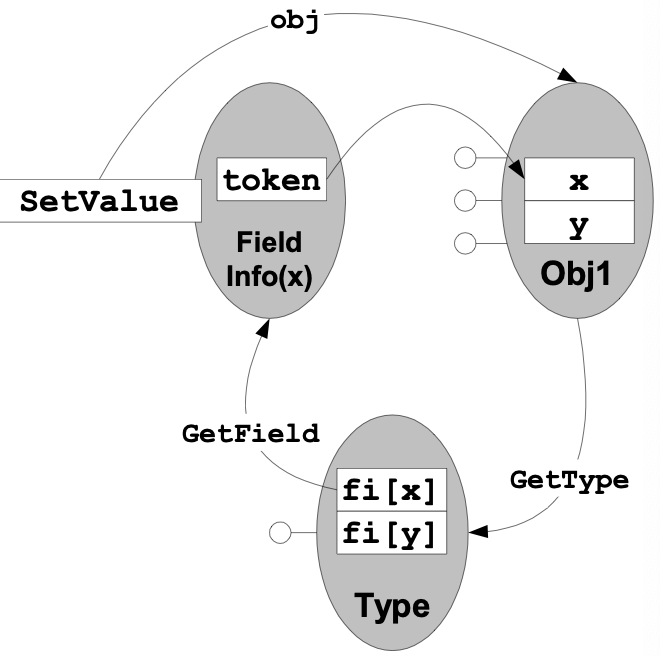
\includegraphics[scale=.3]{graphic/ref attr/field info.png}
\end{center}
\vspace{-8pt}
\begin{lstlisting}
Type type = typeof (Counter);
Counter c = new Counter(1);

// All Fields
FieldInfo[] fiAll = type.GetFields(
    BindingFlags.Instance |
    BindingFlags.NonPublic);

// Specific Field
FieldInfo fi = type.GetField(
    "countValue",
    BindingFlags.Instance |
    BindingFlags.NonPublic);

int val01 = (int) fi.GetValue(c);
c.Increment();
int val02 = (int) fi.GetValue(c);

fi.SetValue(c, -999);
\end{lstlisting}

\subsubsection{Property Info}
\begin{itemize}
    \item Beschreibt ein Property auf einer Klasse (Name, Typ, etc)
    \item Erlaubt lesen / schreiben eines Feldes
    \begin{itemize}
        \item object GetValue(object obj);
        \item public void SetValue(object obj, object value);
    \end{itemize}
\end{itemize}
\begin{lstlisting}
Type type = typeof(Counter);
Counter c = new Counter(1);

// All Properties
PropertyInfo[] piAll = type.GetProperties();

// Specific Property
PropertyInfo pi = type.GetProperty("CountValue");

int val01 = (int)pi.GetValue(c);
c.Increment();
int val02 = (int)pi.GetValue(c);

if (pi.CanWrite) {
    pi.SetValue(c, -999);
}
\end{lstlisting}

\subsubsection{Method Base}
\begin{itemize}
    \item Basisklasse für MethodInfo und ConstructorInfo
    \item Konstruktoren und Methoden sind aus Sicht der Metadaten recht ähnlich
\end{itemize}

\subsubsection{Method Info}
\begin{itemize}
    \item Beschreibt eine Methode auf einer Klasse (Name, Paramteter, etc.)
    \item Leitet von der Klasse «MethodBase» ab
    \item Kann über «Invoke»-Methode aufgerufen werden
\end{itemize}
\begin{lstlisting}
Type type = typeof(Counter);
Counter c = new Counter(1);

// All Methods
MethodInfo[] miAll = type.GetMethods();

// Specific Method
MethodInfo mi = type.GetMethod("Increment");

mi.Invoke(c, null);
\end{lstlisting}

\subsubsection{Method Info / mit Parametern}
\begin{lstlisting}
Type type = typeof(System.Math);

Type[] paramTypes = { typeof(int) };

// Get method info for Cos(  )
MethodInfo miAbs = type
    .GetMethod("Abs", paramTypes);

// Fill an array with the actual parameters
object[] params = { -1 };

object returnVal = miAbs.Invoke(type, params)
\end{lstlisting}

\subsubsection{Constructor Info}
\begin{itemize}
    \item Beschreibt einen Konstruktoren einer Klasse (Name, Parameter, etc.)
    \item Leitet von der Klasse «MethodBase» ab
    \item Kann über «Invoke»-Methode aufgerufen werden
\end{itemize}
\begin{lstlisting}
Type type = typeof(Counter);

// All Constructors
ConstructorInfo[] ciAll = type.GetConstructors();

// Specific Constructor Overload 01
ConstructorInfo ci01 = type.GetConstructor(
    new[] { typeof(int) });

Counter c01 = (Counter)ci01.Invoke(
    new object[] { 12 });

// Specific Constructor Overload 02
ConstructorInfo ci02 = type.GetConstructor(
    BindingFlags.Instance|BindingFlags.NonPublic,
    null, new Type[0], null);

Counter c02 = (Counter)ci02.Invoke(null);
\end{lstlisting}

\subsubsection{Constructor Info via «Activator»}
\begin{lstlisting}
// Alternative
Counter c03 = (Counter)Activator
    .CreateInstance(
        typeof(Counter), 12 // , "further params", "", ...);

// Alternative
// -> when Public Default Constructor exists
Counter c04 = Activator
    .CreateInstance<Counter>();
\end{lstlisting}
